\documentclass[11pt, a4paper]{article}

\usepackage[T1]{fontenc}
\usepackage[utf8]{inputenc}
\usepackage[UKenglish]{babel}
\usepackage{amsmath}
\usepackage{amsthm}
\usepackage{amssymb}
\usepackage{float}
\usepackage{graphicx}
\usepackage{algorithm}
\usepackage{algorithmic}
\usepackage{todonotes}
\usepackage{enumitem}

\newcommand{\nni}{\mathrm{NNI}}
\newcommand{\rnni}{\mathrm{RNNI}}
\newcommand{\rnniu}{\mathrm{RNNIu}}

\newtheorem{definition}{Definition}
\newtheorem{theorem}[definition]{Theorem}
\newtheorem{conjecture}[definition]{Conjecture}
\newtheorem{lemma}[definition]{Lemma}
\newtheorem{corollary}[definition]{Corollary}

\graphicspath{{figures/}}

\title{The Ranked Nearest Neighbour Interchange space}
\date{\today}
\author{Lena Collienne, Alex Gavryushkin}


\begin{document}

\maketitle

\begin{abstract}

\end{abstract}


\section{Introduction}

%Introduce RNNI as ranked nearest neighbour interchange space, only ultrametric trees considered (extension could be mentioned in the end)

%We use the exact algorithm to calculate all the distances for the examples given in this paper

\section{Definitions}

\todo{citation of definitions??}

A \amph{rooted binary phylogenetic tree} on a set $X$ is a pair $(t, \Phi)$ where $t$ is a rooted binary tree with leaf set $\mathcal{L}(t)$ and $\Phi:X \mapsto \mathcal{L}(T)$ a bijective mapping. \todo{do we need to define leaves and internal nodes, child, parent, subtree, cherry(defined below)?}
From now on, we assume $X = \{1,\ldots,n\}$ for a fixed number $n \in \mathbb N$ of leaves.
Within this paper we study \emph{ranked trees} that are determined by a pair consisting of a rooted binary phylogenetic tree $(t, \Phi)$ on $X = \{1, \ldots, n\}$ for $n \in \mathbb N$, and a rank function.
A \emph{rank function} on $t$ maps the vertex set of $t$ onto the set $\{0,\ldots,n-1\}$ such that all leaves are assigned rank $0$ and each internal node has rank greater than its children.
The rank of a node $v$ in a ranked tree will be denoted by $rank(v)$.
For simplicity of notation we use the term \emph{tree} instead instead of ranked tree.
Furthermore, we will identify leaves by their labels and might call them \emph{taxa} (singular: \emph{taxon}).
For a tree $T$ a subtree consisting of an internal node with both children being leaves is called \emph{cherry}.
An edge $e$ that has no leaf as child is an \emph{internal edge} and we say an edge $e=(u,v)$ has \emph{length} $l$ if ${|rank(v) - rank(u)| = l}$.
Each internal edge defines a \emph{cluster} which is the set of taxa that are descending from the lower of both nodes bounding $e$. \todo{OK?}
In the literature, clusters often refer to sets of taxa descending from internal nodes in which case clusters as defined above coincide with non-trivial clusters.
Given a subset $S$ of the set of taxa $X$, the \emph{most recent common ancestor} $mrca(S)$ of $S$ is the internal node with lowest rank that is ancestor of all taxa in $S$. \todo{OK?}
In particular, for a single taxon $x \in X$, $mrca(\{x\})$ is the parent of $x$ and will be denoted by $parent(x)$.
We write $mrca_T(S)$ to emphasise that we consider the most recent common ancestor of set $S$ in tree $T$.
Two trees are called \emph{isomorphic} if the underlying rooted phylogenetic trees are isomorphic and the isomorphism preserves ranks of the nodes.

Now we are ready to define the tree space that is the subject of study of this paper, the $\rnni$ graph.
The vertex set of the \emph{$\rnni$-graph} is given by the set of all ranked trees on $n$ taxa.
We introduce two types of operations (\emph{$\rnni$ moves}) connecting trees $T$ and $R$ in this graph by an edge:
The swap of the ranks of two internal nodes that have rank difference one is called \emph{rank move}.
We say that there is an $\nni$ move between trees $T$ and $R$ if there are edges $e$ in $T$ and $f$ in $R$ that are bounded by internal nodes with rank difference one such that the graphs obtained by shrinking $e$ and $f$ to internal nodes are isomorphic.
Trees that are connected by either a rank move or an $\nni$ move are called \emph{$\rnni$ neighbours} or briefly neighbours.
Note that the previously defined $\rnni$ graph is a metric space, which is why we may call it \emph{$\rnni$ space} or just $\rnni$.

\todo{figure: rank + $\nni$ move}

The main purpose of this paper is understanding geometric properties of the $\rnni$ space.
Therefore, further notations need to be introduced.
If every internal node of a tree $T$ has at least one child that is a leaf, $T$ is called \emph{caterpillar tree}.
A \emph{path} $p$ between trees $T_0$ and $T_m$ in $\rnni$ is a sequence $T_0, T_1, \ldots, T_m$ of trees such that there is an edge $\{T_i, T_{i+1}\}$ for all $i=0,\ldots,m-1$.
For such a path $p$ we say the \emph{length} $|p|$ of $p$ is $m$.
A path $p$ between trees $T$ and $R$ is a \emph{shortest path} if for every path $r$ between $T$ and $R$, $|p| \leq |r|$.
The \emph{distance} $d(T,R)$ between trees $T$ and $R$ is the length of a shortest path between them.
If $p$ is a path only consisting of caterpillar trees we call it \emph{caterpillar path}.
For two caterpillar trees $T$ and $R$ a \emph{shortest caterpillar path} is a caterpillar path that is shortest among all caterpillar paths between $T$ and $R$.
The length of such a shortest caterpillar path is called \emph{caterpillar distance} and denoted by $d_c(T,R)$.
A set $\mathbb S$ of trees is called \emph{convex} if for all pairs of trees $T,R \in \mathbb S$, there exists a shortest path from $T$ to $R$ such that every tree on $p$ is element of $\mathbb S$.

%Is it sufficient to mention what RNNI stands for in the Introduction?

%Restrict to RNNIu (See whether we can get same results for RNNI)

%Definitions inside a tree: cherry, partition, edges represent partitions

%If needed: diameter, radius (in the corresponding chapter?), induced triplet (in that chapter?)

%delete definitions in the following chapters that are already covered here!


%replace rank swap with rank move in the following!!

\section{Geometry of $\rnni$}

The following Algorithm~\ref{alg:find_path} which computes paths between pairs of trees in $\rnni$ is a central tool for our investigation of shortest paths in $\rnni$.

\begin{algorithm}[H]
\caption{FIND\_PATH($T,R$)}
\label{alg:find_path}
\begin{algorithmic}[1]
	\STATE $\hat{T} := T$
	\STATE $p := (T)$
	\FOR {$i = 1, \dots, n-2$}
		\STATE Let $C$ be the cluster associated with edge $(v,w)$ in $R$ with ${rank(v) = i < rank(w)}$
		\WHILE {$rank(mrca_{\hat{T}}(C))>i$}
			\STATE Update $\hat{T}$: Decrease $rank(mrca_{\hat{T}}(C))$ by an $\rnni$ move \label{alg:line:move_set_down}
			\STATE $p = p+\hat{T}$
		\ENDWHILE
	\ENDFOR
	\RETURN $p$
\end{algorithmic}
\end{algorithm}

\todo{figure of an example?}

One can easily prove that there is always exactly one $\rnni$ move on $T$ that decreases the rank of $mrca_T(C)$ as in line~\ref{alg:line:move_set_down} of Algorithm~\ref{alg:find_path}.
It follows that Algorithm~\ref{alg:find_path} returns a path in $\rnni$ for any pair of trees $T,R$.
Moreover, it gives an upper bound for the diameter of $\rnni$, which improves the one given in~\cite{Gavryushkin2017}:

\begin{lemma}
    It is $\Delta(\rnni) \leq \frac{(n-1)(n-2)}{2}$.
\end{lemma}

\begin{proof}
    Let us consider the maximum length of a path given by Algorithm~\ref{alg:find_path}.
    In worst case each of the $n-2$ clusters $C$ given by internal edges of $R$, represented by $i = 1, \dots, n-2$ in the algorithm, requires $n-1-i$ $\rnni$ moves for moving $mrca(C)$ down in $\hat{T}$.
	Hence, the maximum length of a path computed by that algorithm for any pair of trees is less or equal to ${\sum\limits_{i = 1}^{n-2} i = \frac{(n-2)(n-1)}{2}}$.
\end{proof}

Lemma~\ref{lemma:distance_delete_taxon} is central for some of the following induction proofs. \todo{Is it correct and if it is, do we need to prove the statement, or is it rather obvious?}

\todo{Change notations in this lemma+proof (less indices!!)}
\begin{lemma}
    Let $T_1$ and $T_2$ be two trees on $n+1$ taxa.
    Let $T_1|_n$ and $T_2|_n$ be these trees restricted to $n$ taxa, i.e. the same taxon $n+1$ is deleted from both trees $T_1$ and $T_2$.
    Then it is $d(T_1|_n, T_2|_n) \leq d(T_1,T_2) - |r_{T_1}(p_{n+1}) - r_{T_2}(p_{n+1})|$ where $r_{T_i}(p_j)$ determines the rank of the parent of taxon $j$ in tree $T_i$.
    \label{lemma:distance_delete_taxon}
\end{lemma}

\begin{proof}
    Induction on $k = d(T_1,T_2)$:

    Basis($k = 1$):
    If rank of $p_{n+1}$ changes between $T_1$ and $T_2$, it is $d(T_1|_n, T_2|_n) = 0$ and $|r_{T_1}(p_{n+1}) - r_{T_2}(p_{n+1})| = 1$ and therefore, $d(T_1|_n, T_2|_n) = 0 \leq 1 - 1 = d(T_1,T_2) - |r_{T_1}(p_{n+1}) - r_{T_2}(p_{n+1})|$.
    If on the other hand the rank of $p_{n+1}$ does not change between $T_1$ and $T_2$, it is $d(T_1|_n, T_2|_n) = d(T_1,T_2) = 1$ and $|r_{T_1}(p_{n+1}) - r_{T_2}(p_{n+1})| = 1$ and therefore, $d(T_1|_n, T_2|_n) = 1 \leq 1 - 0 = d(T_1,T_2) - |r_{T_1}(p_{n+1}) - r_{T_2}(p_{n+1})|$.

    Step($k \to k+1$):
    Let $T_1$ and $T_2$ be trees on $n+1$ taxa with distance $d(T_1,T_2) = k$.
    Let $T_2'$ be the last tree on a shortest path from $T_1$ to $T_2$, i.e. $d(T_1,T_2') = k$.
    We can apply the induction hypothesis on $T_1$ and $T_2'$ and see that $d(T_1|_n, T_2'|_n) \leq d(T_1, T_2') - |r_{T_1}(p_{n+1}) - r_{T_2'}(p_{n+1})| := k - m$.
    Now we differ two cases:
    \begin{enumerate}
        \item $p_{n+1}$ changes its rank between $T_2$ and $T_2'$ or is affected by the $\nni$ move is performed between $T_2$ and $T_2'$.

        Then the trees $T_2|_n$ and $T_2'|_n$ are equal. \todo{Is this obivous?}
        Therefore, it is $d(T_1|_n,T_2|_n) = d(T_1|_n, T_2'|_n) \leq k - m$.
        It is either $|r_{T_1}(p_{n+1}) - r_{T_2}(p_{n+1})| = m+1$, $|r_{T_1}(p_{n+1}) - r_{T_2}(p_{n+1})| = m$, or $|r_{T_1}(p_{n+1}) - r_{T_2}(p_{n+1})| = m-1$.
        In either case, we have $d(T_1|_n,T_2|_n) = d(T_1|_n, T_2'|_n) \leq k - m = (k+1) - (m+1) \leq d(T_1, T_2) - |r_{T_1}(p_{n+1}) - r_{T_2}(p_{n+1})|$.

        \item $p_{n+1}$ has same rank in $T_2$ and $T_2'$.

        In this case it is $d(T_1|_n,T_2|_n) \leq d(T_1|_n,T_2'|_n) + d(T_2'|_n, T_2|_n) \leq d(T_1|_n, T_2'|_n) + 1 \leq (k-m)+ 1$.
        It also follows that $|r_{T_1}(p_{n+1}) - r_{T_2'}(p_{n+1})| = |r_{T_1}(p_{n+1}) - r_{T_2}(p_{n+1})|$ and therefore, we can conclude $d(T_1|_n,T_2|_n) \leq k-m+1 = k+1-m = d(T_1,T_2) -  |r_{T_1}(p_{n+1}) - r_{T_2}(p_{n+1})|$.
    \end{enumerate}
\end{proof}


\subsection{The set of caterpillar trees}
\label{section:caterpillar_convex}

The set of caterpillar trees is of interested in $\rnni$ because shortest paths between such trees in $\rnni$ differ from those in classical $\nni$ space.
Since $\nni$ moves in $\rnni$ are only allowed on edges of length one, the structure of shortest paths between caterpillar trees is different in $\nni$ and $\rnni$ as it is pointed out in Figure~\ref{fig:NNI_vs_RNNI}.

\begin{figure}[H]
	\centering
	\includegraphics[width=\textwidth]{NNI_vs_RNNI}
	\caption{Paths between caterpillar trees $T$ and $R$: black -- shortest path in classical $\nni$ (ignoring ranks) of length $5$; red -- shortest path in $\rnni$ of length $6$; blue -- path in $\rnni$ which is the natural extension of the shortest path in $\nni$ but has length $8$.}
	\label{fig:NNI_vs_RNNI}
\end{figure}

This observation already suggests that there is always a caterpillar path that is shortest path between two arbitrary caterpillar trees in $\rnni$.
Indeed, our aim for this section is to prove Theorem~\ref{thm:caterpillar_convex} which states that the set of caterpillar trees is convex in $\rnni$.
Note that this is not true for the $\nni$ space, which is clear from the example in Figure~\ref{fig:NNI_vs_RNNI}.

% Shall we mention the data structure we use (list of sets) - this might be useful to see the connection to the partition lattice.
One can see caterpillar trees as sequences of taxa, ordered non-decreasing according to the ranks of their parents.
$\nni$ moves between caterpillar trees, which are the only possible $\rnni$ moves between caterpillar trees, coincide with exchanges of two neighboured elements in the sequence.
In these sequences the first two taxa are somehow equivalent since they build the unique cherry.
$\nni$ moves that change the cherry of a tree refer to exchanges of the first or the second element with the third element of the sequence while exchanges of the first two elements do not change the corresponding tree.
With this observation we can provide an algorithm for computing shortest caterpillar paths by a simple modification of the commonly known \emph{Bubble Sort} algorithm~\cite{knuth1997}:

Following the observations above, only the moves for the first three positions of a sequence with Bubble Sort need to be adapted for the computation of shortest caterpillar paths.
Let us consider the first three elements $a,b,c$ which appear in this order in a sequence representing a caterpillar tree on a caterpillar path between trees $T$ and $R$.
If the rank of $parent(c)$ is higher than the ranks of $parent(a)$ and $parent(b)$ in $R$, there are no swaps needed for these taxa.
If just one of the two taxa $a$ and $b$ is on the other side of $c$ in $R$, this one swaps position with $c$ in the sequence.
But if both $a$ and $b$ are on the other side of $c$ in $R$, the one that has the parent with highest rank of all these three taxa in $R$ swaps with $c$ at first.
This makes sure that there is no additional swap of $a$ and $b$ needed on the path to $R$.

Lemma~\ref{lemma:caterpillar_dist=diameter} regards caterpillar trees with distance $\frac{(n-1)(n-2)}{2}$ and will be needed for proving the convexity of the set of caterpillar trees in $\rnni$.

\begin{lemma}
    Let $T$ and $T'$ be two caterpillar trees.
    $T$ and $T'$ have distance $d(T,T') = \Delta(\rnniu) = \frac{(n-1)(n-2)}{2}$ if, and only if, they have caterpillar distance $d_c(T,T') = \Delta(\rnniu) = \frac{(n-1)(n-2)}{2}$. \todo{define $d_c$}
    \label{lemma:caterpillar_dist=diameter}
\end{lemma}

    % \todo{At the top of $T'$ it could also be $2,1$, or $t=1$}
    %
    % \begin{figure}[H]
    %     \centering
    %     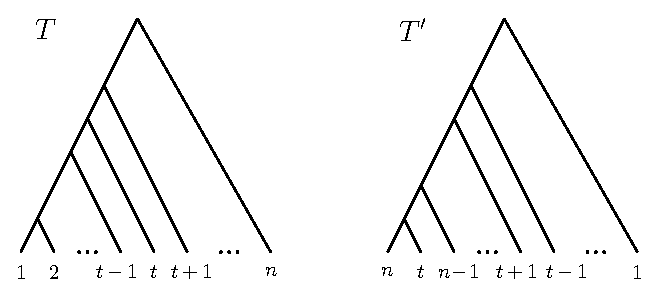
\includegraphics[width=0.6\textwidth]{caterpillar_max_dist}
    %     \caption{Caterpillar trees $T$ and $T'$ with distance $d(T,T') = \Delta(\rnniu)$}
    %     \label{fig:caterpillar_max_distance}
    % \end{figure}

\begin{proof}
    Let $d_c(T,T')$ denote the length of a shortest caterpillar path from $T$ to $T'$, that is a caterpillar path that is shortest among all caterpillar paths from $T$ to $T'$.
    We need to prove that $d(T,T') = \Delta(\rnniu)$ if, and only if, $d_c(T,T') = \Delta(\rnniu)$.

    Let $T$ and $T'$ have distance $d(T,T') = \Delta(\rnniu)$.
    We can compute a  shortest caterpillar path from $T$ to $T'$ using Bubble Sort.
    In each loop $k=1, \ldots, n-2$ of the algorithm there can be at most $n-1-k$ exchanges of taxa.
    It follows that the maximum length of a path computed by Bubble Sort is $\sum\limits_{k=1}^{n-2} k = \frac{(n-1)(n-2)}{2}$.
    Since there cannot be a caterpillar path shorter than $\frac{(n-1)(n-2)}{2}$ if it is $d(T,T') = \frac{(n-1)(n-2)}{2}$, it follows $d_c(T,T') = \Delta(\rnniu)$.

    Let now $T$ and $T'$ have caterpillar distance $d_c(T,T') = \Delta(\rnniu)$.
    We prove $d(T,T') = d_c(T,T')$ by induction on the number of taxa $n$ of $T$ and $T'$:
    We assume without loss of generality that $T$ is the caterpillar tree $(\ldots ((1,2),3), \ldots, n)$.
    Otherwise, we re-label $T$ and $T'$.
    Let $T'$ be a caterpillar tree with distance $\Delta(\rnniu)$ to $T$.

    Induction basis: $n=3$\\
    All trees have distance $1$ and are caterpillar trees.

    Induction step: $n \to n+1$\\
    Induction hypothesis: For trees $R$, $R'$ on $n$ taxa it is $d_c(R,R') = d(R, R') = \frac{(n-1)(n-2)}{2} = \Delta(\rnniu_n)$.\\
    Let $T, T'$ be trees on $n+1$ taxa with caterpillar distance $\Delta(\rnniu_{n+1})$.
    When applying the Bubble Sort algorithm to compute a path between $T'$ and $T$, each pair of taxa that is compared in that algorithm exchanges, since there must be $\Delta(\rnniu)=\frac{(n-1)(n-2)}{2}$ moves between $T$ and $T'$.
    So we can conclude that taxon $n+1$ must be in the cherry of $T'$.
    Let us consider the trees $T|_n$ to $T'|_n$ that result from $T$ and $T'$ by deleting taxon $n+1$.
    When running Bubble Sort to compute a path from $T|_n$ to $T'|_n$ one can observe the same exchanges of taxa as on the Bubble Sort path from $T$ to $T'$, except for the $n-1$ ones that involve taxon $n+1$.
    Hence, the caterpillar distance is $d_c(T|_n, T'|_n) = \frac{n(n-1)}{2} - (n-1)$ = $\frac{(n-1)(n-2)}{2}$.
    So we can apply the induction hypothesis on $T|_n$ and $T'|_n$ and know that $d(T|_n,T'|_n) = \frac{(n-1)(n-2)}{2}$.

    With Lemma~\ref{lemma:distance_delete_taxon} we know that the distance between $T|_n$ and $T'|_n$ is at least $d(T|_n, T'|_n) \leq d(T,T') - |r_{T}(p_{n+1}) - r_{T'}(p_{n+1})|$.
    We also know $|r_{T}(p_{n+1}) - r_{T'}(p_{n+1})| = n-1$
    If we assume that there is a path from $T$ to $T'$ of length less than $\Delta(\rnniu_{n+1}) = \frac{n(n-1)}{2}$, it would follow that $d(T|_n, T'|_n) \leq d(T,T') - |r_{T}(p_{n+1}) - r_{T'}(p_{n+1})| < \frac{n(n-1)}{2} - (n-1) < \frac{(n-1)(n-2)}{2}$.
    So it would be $d(T|_n, T'|_n) < \Delta(\rnniu_n)$.
    Since this is a contradiction to $d(T|_n, T'|_n) = \Delta(\rnniu_n)$, it must be $d(T,T') = \Delta(\rnniu_{n+1}) = \frac{n(n-1)}{2} $.

\end{proof}

\begin{theorem}
    The set of caterpillar trees is convex.
    \label{thm:caterpillar_convex}
\end{theorem}

\begin{proof}
    We prove the Theorem by backwards induction on the length $l$ of a shortest caterpillar path between two caterpillar trees $T$ and $T'$.

    Induction basis: $l = \Delta(\rnniu) = \frac{(n-1)(n-2)}{2}$\\
    With Lemma~\ref{lemma:caterpillar_dist=diameter} one can see that for each pair of caterpillar trees $T$, $T'$ with caterpillar distance $d_c(T,T') = \Delta(\rnniu)$, it is $d(T,T') = d_c(T,T')$, which means that there is a shortest path between $T$ and $T'$ that is a caterpillar path.

    Induction step: $l+1 \to l$\\
    Induction hypothesis: For each pair of caterpillar trees with caterpillar distance $l+1$ there is a shortest path between these trees that only consists of caterpillar trees, which means that the distance between these trees is $l+1$.
    Let $T$ and $T'$ be caterpillar trees with caterpillar distance $l$.
    Since $l < \Delta(\rnniu) = \frac{(n-1)(n-2)}{2}$, there is one loop $k$ in the Bubble Sort algorithm from $T'$ to $T$ where there are less than $n-2-k$ swaps of neighboured taxa.
    This means that there is a taxon $a$ that has parent with rank $n-2-k$ in $T$ and that does not need to move all the way up starting at the cherry in loop $k$.
    Therefore, there must be a taxon $b$ which has parent with rank one less than the parent of $a$ in the tree at the beginning of loop number $k$.
    If we assume that loop $k$ is the first loop where a single taxon is not moved by $n-k-2$ $\rnni$ moves, it follows that $a$ and $b$ must be neighboured taxa in $T'$.
    Let $T''$ be the caterpillar tree resulting from $T'$ by exchanging $a$ and $b$.
    It follows that $T'$ has caterpillar distance $d_c(T,T'') = d_c(T,T') + 1 = l+1$ to $T$ and $d(T',T'') = 1$.
    We can apply the induction hypothesis on $T$ and $T''$ and know that $d(T,T'') = l+1$.
    If it was $d(T,T') < l$, it would hold $d(T,T'') \leq d(T,T') + d(T',T'') < l + 1$ which contradicts the induction hypothesis.
    We can conclude that $d(T,T') = l$.

\end{proof}


\subsection{Diameter}

In~\cite{Gavryushkin2017} upper and lower bound for the diameter of $\rnni$ are given.
Following the results of section~\ref{section:caterpillar_convex} one can directly improve this result by giving the exact diameter of the $\rnni$ graph.

\begin{lemma}
	There are two caterpillar trees in $\rnniu$ with distance $\frac{(n-1)(n-2))}{2}$.
	\label{conj:caterpillar_diameter}
\end{lemma}

\begin{proof}
	Let $T = (( \dots (n,1)2)\dots)n-1)$ and $R = (( \dots (n,n-1)n-2)\dots)1)$.
    According to Theorem~\ref{thm:caterpillar_convex}, there is a shortest path between $T$ and $R$ that is a caterpillar path.
    We can compute a shortest caterpillar path by using the modified version of Bubble Sort as explained above. \todo{Do we want to name this algorithm?}
    When running this algorithm on $T$ and $R$, taxon $i$ swaps $n-1-i$ times with its right neighbour.
    Therefore, the length of a shortest caterpillar path is ${\sum\limits_{i=1}^{n-1}(n-1-i) = \sum\limits_{i=0}^{n-2}i = \frac{(n-1)(n-2)}{2}}$.
\end{proof}

\begin{corollary}
    It is $\Delta(\rnniu) = \frac{(n-1)(n-2)}{2}$.
\end{corollary}

%Do we need this?

% \begin{lemma}
% 	Let $T_1$ and $T_2$ be two caterpillar trees that both have a leaf labelled by $a$ as part of their cherry.
% 	There is a shortest paths from $T_1$ to $T_2$ that is a caterpillar path.
% 	\label{lemma:caterpillar_subset_convex}
% \end{lemma}
%
% \begin{figure}[h]
% 	\centering
% 	\includegraphics[width=0.3\textwidth]{label_internal_nodes}
% 	\caption{The labelling of the caterpillar tree as introduced in the proof of Lemma~\ref{lemma:caterpillar_subset_convex} is unique due to its definition.
% 	}
% 	\label{label_internal_nodes}
% \end{figure}
%
% \begin{proof}
% 	Let $T_1$ and $T_2$ be two caterpillar trees, both having a leaf labelled by $a$ as part of their cherry.
% 	Let $p$ be a shortest path from $T_1$ to $T_2$.
% 	We introduce a labelling of internal nodes of all trees on $p$ by first defining it for the caterpillar trees $T_1$ and $T_2$ and then explaining how the labelling is changed by $\rnni$ moves.
%
% 	In $T_1$ and $T_2$ the internal node of the cherry is labelled by the label of its child that is not $a$.
% 	All other internal nodes shall have the same label as their leaf children.
% 	From now on we will identify the leaf labelled by $x$ with $x$ and the internal node labelled by $x$ will be called $int_x$.
% 	An example for a caterpillar tree with internal leaf labels is depicted in Figure~\ref{label_internal_nodes}.
% 	In the following, changes of the internal labelling following $\rnni$ moves are defined:
%
% 	\textbf{Rank moves:}
% 	Within rank moves the labels of internal nodes do not change.
% 	For an example consider Figure~\ref{fig:rank_swap_internal_label}.
%
% 	\begin{figure}[H]
% 		\centering
% 		\includegraphics[width=0.8\textwidth]{rank_swap_internal_label}
% 		\caption{The labelling of the internal nodes that swap ranks (red) do not change within the rank move.
% 		}
% 		\label{fig:rank_swap_internal_label}
% 	\end{figure}
%
% 	\textbf{NNI move:}
% 	Let there be an $\nni$ move on an edge $(int_x, int_y)$ where $rank(int_x) < rank(int_y)$ as in Figure~\ref{fig:nni_moves}.
%
% 	\begin{figure}[H]
% 		\centering
% 		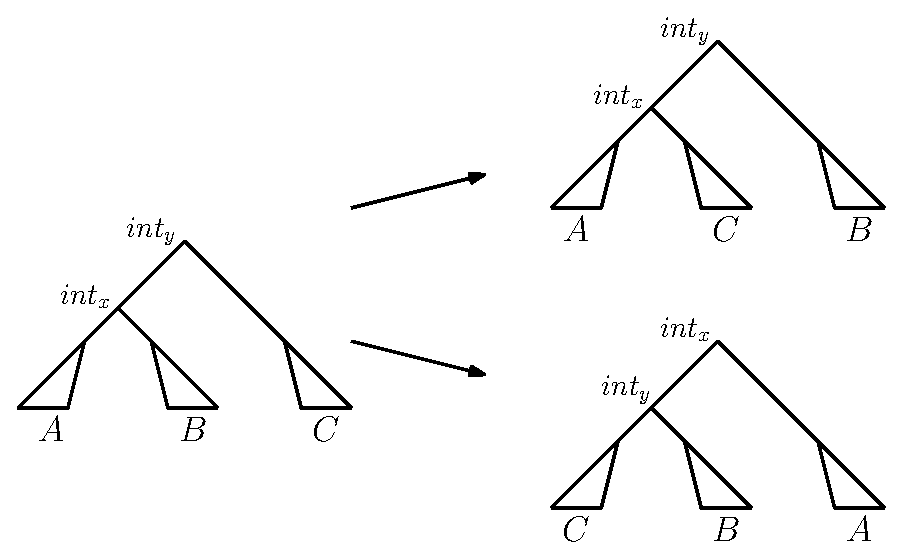
\includegraphics[width=0.7\textwidth]{nni_moves_internal_label}
% 		\caption{Two possible $\nni$ moves on edge $(int_x, int_y)$ where $x \in A, y \in B$.
% 		}
% 		\label{fig:nni_moves}
% 	\end{figure}
%
% 	The nodes incident to the edge after the $\nni$ move are labelled by $int_x$ and $int_y$ as well.
% 	By default, the node that has lower rank than the other one is labelled by $int_x$, the other one by $int_y$.
% 	But if $int_x$ is no ancestor of $x$ or $int_y$ is no ancestor of $y$, we swap the labels of the two new nodes, such that $rank(int_x) > rank(int_y)$.
% 	An example of an $\nni$ move and the new labelling is provided in Figure~\ref{fig:nni_example_internal_label}.
%
% 	\begin{figure}[H]
% 		\centering
% 		\includegraphics[width=0.8\textwidth]{nni_example_internal_label}
% 		\caption{The first labelling after the $\nni$ move preserves the ranks of $int_4$ and $int_6$.
% 		But then $int_6$ is not an ancestor of $6$ any more.
% 		Therefore, $int_4$ and $int_6$ have to change their labels.
% 		}
% 		\label{fig:nni_example_internal_label}
% 	\end{figure}
%
% 	We proceed to show that $int_x$ and $int_y$ are ancestors of $x$ and $y$ after an $\nni$ move as described above, respectively.
% 	If $x$ stays in the subtree rooted in the lower node of $e$, this does obviously hold.
% 	We now turn to the case that $x$ is not in the subtree rooted in the lower node of $e$ after the $\nni$ move.
% 	Then the labels of the two internal nodes change such that $rank(int_x) > rank(int_y)$.
% 	This makes sure that $int_x$ is an ancestor of $x$.
% 	Thus, it remains to prove that $int_y$ is ancestor of $y$.
% 	In particular, we need to show that $y$ is not in the same subtree $A$ as $x$, whose root has the node labelled by $int_x$ as parent before and after the $\nni$ move.
% 	Let us consider the tree before the $\nni$ move.
% 	$A$ has $|A|$ leaves and $|A| - 1$ internal nodes.
% 	These internal nodes are labelled by some leaves of $A$, because all internal nodes must be labelled by a descendant leaf.
% 	We know that $x \in A$, and the parent of the root of $A$ is labelled by $x$.
% 	All remaining $|A|-1$ leaf labels of $A$ appear as labels of the $|A|-1$ internal nodes of $A$.
% 	From the fact that the internal node labelled by $y$ is not inside $A$ we can conclude that $y$ cannot be a leaf of $A$.
% 	This proves that the labelling of the internal nodes is is well defined and allows a unique identification of internal nodes by their labels.
%
% 	The task is now to prove that there is always a caterpillar path at least as short as the given path $p$.
% 	Therefore, we use the following observation:
% 	Within each $\rnni$ move the ranks of at most two internal nodes change by at most one each.
% 	This is true for both rank moves and $\nni$ moves, according to our definition of the labelling:
% 	Within a rank move two nodes exchange their ranks, while there are not necessarily changes of ranks when $\nni$ moves are performed.
%
% 	On a caterpillar path the only possible moves are $\nni$ moves that change the ranks of two internal nodes by one each.
% 	Therefore, we can construct a caterpillar path $r$ out of $p$:
% 	every time two internal nodes $int_x$ and $int_y$ exchange ranks on $p$, they do so on the caterpillar path $r$ as well.
% 	Since there are moves on $p$ that do not change the ranks of internal nodes, this caterpillar path has length $|r| \leq |p|$.
% 	Hence, there is always a shortest path between $T_1$ and $T_2$ that is a caterpillar path.
% \end{proof}

\subsection{Split Theorem}

When analysing the complexity of the $\rnni$ space, the comparison to $\nni$ is an important step.
The proof of NP-completeness of $\nni$ in~\cite{jiang2000} is based on the fact that following theorem holds in $\nni$.

\begin{theorem}
	There are trees $T_1,T_2$ in $\nni$ sharing a partition which is not shared by any intermediate tree on a shortest path from $T_1$ to $T_2$.
	\label{thm:split_nni}
\end{theorem}

\begin{proof}
	See~\cite{Li1996}.
\end{proof}

The proof presented in~\cite{Li1996} for Theorem~\ref{thm:split_nni} does not work for $\rnni$.

%This part is mainly for myself, not sure whether it is important to have it in the paper
The counterexample presented in~\cite{Li1996} works in $\nni$ is based on following observation:
Let $T_1$ and $T_2$ be two caterpillar trees.
If each taxon $a$ is replaced by a cherry $(a_1,a_2)$ in both trees $T_1$ and $T_2$, the resulting trees $T_1'$ and $T_2'$ have distance $d_{\nni}(T_1',T_2') = d_{\nni}(T_1,T_2)$ in the $\nni$ graph.
When proving~\ref{thm:split_nni},~\cite{Li1996} give an example of two trees $T$ and $R$ on $2n$ taxa that consist of two caterpillar trees each that share the root as parent.
The split given by the edges incident to the root is $1, \ldots, n | n+1, \ldots, 2n$ in both trees $T$ and $R$.
For the given example there is a shortest path in $\nni$ where at first $T$ is transformed to a tree $T'$ with $n$ cherries where each cherry contains one taxon of $\{1, \ldots, n\}$ and one taxon of $\{n+1, \ldots, 2n\}$.
Afterwards, $T'$ is tranformed to a tree $R'$ that contains the same cherries as $T'$.
Finally, all cherries of $R'$ are resolved in order to end up in tree $R$.
For proving that this path is shorter than any path preserving the split $1, \ldots, n | n+1, \ldots, 2n$, the fact that $d_{\nni}(T',R') = d_{\nni}(T|_{\{1, \ldots, n\}}, R|_{\{1, \ldots, n\}})$ is being used.
However, this does not work in $\rnni$.
Introducing new cherries means introducing new internal nodes with new ranks.
Since there are some rank moves needed for an $\rnni$ path similar to the shortest $\nni$ path presented above, the path in $\rnni$ that breaks the split $1, \ldots, n | n+1, \ldots, 2n$ is no shortest path.
% How do we assign the ranks to the new cherry nodes?
% We could either create a path where $T'$ and $R'$ have distance equal to $d_{\rnni}(T|_{\{1, \ldots, n\}}, R|_{\{n+1, \ldots, 2n\}})$ and have a lot of additional rank moves before and after that part OR
% Build $T'$ and $R'$ that contain all the cherries within the least number of moves possible (3n-3) and having a longer path between $T'$ and $R'$.
% Also anything in between these two options is possible. Are we able to disprove every option??


Therefore, the following conjecture was raised~\cite{Gavryushkin2017}.

\begin{conjecture}[Split Theorem]
	For the $\rnni$ graph the following statement holds:
	If a partition of leaves given by an edge is present in two trees $T$ and $R$ then the partition is presented in every tree on every shortest path between $T$ and $R$.
	\label{split_theorem}
\end{conjecture}

However, we found a counterexample to this conjecture:

\begin{figure}[H]
	\centering
	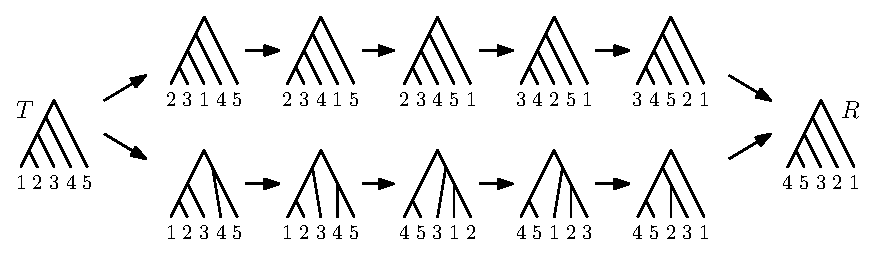
\includegraphics[width=\textwidth]{splitthm_counterexample}
	\caption{The split $123|45$ is present in $T_1$ and $T_2$, but the path at the top is a shortest path where none of the trees contains this split.
    However, this split is maintained on the path at the bottom that is a shortest path as well.}
	\label{splitthm_counterexample}
\end{figure}

Since the counterexample in Figure~\ref{splitthm_counterexample} clearly shows that the version of the Split Theorem stated in~\cite{Gavryushkin2017} does not hold, we will now claim an alternative to this conjecture.
The alternative formulation is based on the observation that there is a shortest path preserving all splits between the trees of the counterexample of the Split Theorem, which is presented at the bottom of Figure~\ref{splitthm_counterexample}.


\begin{conjecture}[Weak Split Theorem]
	For $\rnni$ graph the following statement holds:
	if a partition of leaves given by an edge is present in two trees $T$ and $R$ then there exists a shortest path between $T$ and $R$ where this partition is present in every tree on this path.
	\label{split_theorem_weak}
\end{conjecture}

\todo{Do we want to keep the weak version of the split thm? It is stronger than the Cluster Thm!}

% The weak Split Theorem (in the version as in Lena's thesis) is computationally proven to hold for trees with up to $6$ taxa ($\sim 38$ min running time on laptop).

Another alternative formulation of the Split Theorem is the \emph{Cluster Theorem}, which considers clusters instead of splits.
Considering clusters rather than splits is more reasonable since two rooted trees have the same set of clusters if, and only if, they are isomorphic~\cite{steel2016}.
The trees $T_1, T_2$ of counterexample~\ref{splitthm_counterexample} share the same set of induced splits, but have distinct sets of clusters.

\begin{conjecture}[Cluster Theorem]
	For the $\rnni$ graph the following statement holds:
	if two trees $T$ and $R$ contain the same cluster $C$, then $C$ is present as cluster in every tree on every shortest path between $T$ and $R$.
	\label{cluster_theorem}
\end{conjecture}


\section{Ideas}
\todo{Which ideas do we want to keep? Shall this become an 'open problems/future work' section?}

Following are some ideas that did not lead to major results so far:
% idea for description of max distance caterpillar trees:

\begin{lemma}
    Let $T_1$ and $T_2$ be caterpillar trees.
    It is $d_c(T_1,T_2) = \Delta(\rnniu)$ if, and only if, $T_1$ and $T_2$ share no induced triplet.
    \todo{define induced triplets}
\end{lemma}

This Lemma does only hold for caterpillar trees and not for trees with more than one cherry.
Furthermore, triplets do not represent ranked trees uniquely as they do not contain information about the ranks of internal nodes (but they can uniquely define caterpillar trees as these only have one cherry)

\begin{proof}
    % Insert the proof here
    Fix $T_1 = (\ldots(1,2) \ldots ,n)$, use induction on $n$ and bubble sort (taxon $n$ must be in cherry of $T_2$ if distance is max).
\end{proof}

\begin{conjecture}
    Let $T_1$ and $T_2$ be trees on $n$ taxa.
    It is $d(T_1,T_2) = \Delta(\rnniu)$ if, and only if, $T_2$ can be produced from $T_1$ by applying Algorithm~\ref{alg:max_dist_tree}.
\end{conjecture}

According to Algorithm~\ref{alg:max_dist_tree}, the number of trees with maximum distance to a given tree $T$ depends on the number of cherries of $T$ and the ranks of their internal nodes.
For caterpillar trees it is $(n-1)!$.
The number of caterpillar trees with distance $\Delta(\rnniu)$ from a given caterpillar tree is $2^{n-2}$.

\begin{algorithm}[H]
\caption{MAX\_DISTANCE\_TREE($T$)}
\label{alg:max_dist_tree}
\begin{algorithmic}[1]
	\STATE $R$ only contains cherry taxa $(a,b)$ of $T$ and has internal node with rank $n-1$
    \STATE In list $L$ all taxa $\{1,\ldots,n\}\setminus\{a,b\}$ are sorted such that the ranks of their parents in $T$ do not decrease
	\FOR {taxon $a$ in $L$}
		\STATE Add an internal node as parent of $a$ on any edge in $R$ such that the new internal node has rank one less than the previously lowest internal node
	\ENDFOR
	\RETURN $R$
\end{algorithmic}
\end{algorithm}

\begin{lemma}
    Let $T$ and $R$ be trees.
    Algorithm~\ref{alg:find_path} gives a path of length $\frac{(n-1)(n-2)}{2}$ between $T$ and $R$ if, and only if, $R$ can be generated from $T$ by applying Algorithm~\ref{alg:max_dist_tree}.
\end{lemma}

%If this is true, we can follow that radius = diameter


\subsection{Partition lattice}

% Define Partition Lattice $\Pi_n$ and max chains in that lattice!

\begin{theorem}
	The $\rnni$ space on $n$ taxa is isomorphic to the space of maximum chains of the partition lattice $\Pi_n$ where two maximum chains are connected by an edge if, and only if, they differ by exactly one partition.
\end{theorem}

\bibliographystyle{abbrv}
\bibliography{lit}

\end{document}
